\documentclass[11pt]{article}
\usepackage[margin=1in]{geometry}
\usepackage{booktabs}
\usepackage{graphicx}
\usepackage{natbib}
\usepackage{hyperref}
\usepackage{amsmath}

\title{Nowcasting Inflation with the Bangla Economic Narrative Index:\\ Local-Language News as a High-Frequency Economic Indicator}
\author{Ann Naser Nabil}
\date{\today}

\begin{document}
\maketitle

\begin{abstract}
This paper evaluates whether the Bangla Economic Narrative Index (BENI), a local-language news-based measure of economic narratives in Bangladesh, improves monthly inflation nowcasting. Using the current TF-IDF BENI prototype from Paper 3, I compare autoregressive inflation forecasts against BENI-augmented models in a recursive pseudo-real-time evaluation from 2018 to 2020. The preliminary evidence is deliberately mixed. BENI is strongly correlated with headline CPI inflation in levels, but the current index does not materially improve same-month or one-month-ahead nowcasts over an autoregressive benchmark. At the three-month horizon, the AR+BENI model produces a small RMSE improvement. These results should be interpreted as a placeholder test of the nowcasting framework, not the final estimate of BENI's value, because the final Paper 3 BanglaBERT index and human-verified labels are still pending.
\end{abstract}

\section{Introduction}

Inflation monitoring in Bangladesh faces a timing problem. Official CPI data arrive with delay, informal activity is large, and price pressure is often visible in local-language public discourse before it appears in formal statistical releases. A Bangla-language news index may therefore provide a high-frequency proxy for expectation pressure, household burden, and institutional stress.

This paper asks whether BENI improves inflation nowcasting relative to models using only autoregressive inflation dynamics. The central policy question is practical: if a central bank had access to a local-language economic narrative dashboard, would its inflation nowcasts improve?

The current version of the paper implements the empirical design using the TF-IDF BENI prototype. The results are intentionally reported as provisional. They are useful because they establish the evaluation pipeline, reveal where the first index does and does not help, and define the benchmark that the final BanglaBERT BENI index must beat.

\section{Related Work}

The paper connects three literatures. The first is inflation nowcasting and short-horizon macroeconomic forecasting, where autoregressive and factor-augmented models are common baselines. The second is news-based nowcasting, where high-frequency text can proxy economic conditions. The third is multilingual and developing-economy economic measurement, where local-language data can capture information absent from English-language business media.

For Bangladesh, the local-language channel is especially relevant. Bangla news may capture price anxiety, exchange-rate concerns, market shortages, and household welfare narratives that English-language outlets cover less consistently.

\section{Data}

\subsection{BENI}

The current empirical run uses the Paper 3 TF-IDF BENI output located at:

\begin{quote}
\texttt{beni/experiment/outputs/index/narrative\_index.csv}
\end{quote}

The index covers 76 usable monthly observations after merging with CPI and lag construction, from September 2014 through December 2020. The main BENI variables are monthly mean economic probability and the monthly share of articles classified as economic.

\subsection{Inflation and Controls}

Headline CPI is loaded from the IMF CPI file already stored in the repository. The target variable is year-on-year log CPI inflation:

\[
\pi_t = 100 \times \left(\log(CPI_t) - \log(CPI_{t-12})\right).
\]

The control variable is year-on-year BDT/USD exchange-rate change from the BIS monthly end-of-period series.

\section{Methods}

\subsection{Recursive Pseudo-Real-Time Forecasting}

For each test origin from January 2018 to December 2020, models are estimated using target observations available up to the previous month. Forecasts are generated for horizons $h \in \{0,1,3\}$. This mimics a real-time nowcasting setting where same-month BENI is observable before official CPI is finalized.

\subsection{Models}

The implemented models are:

\begin{itemize}
  \item M1: autoregressive benchmark using three lags of year-on-year inflation.
  \item M2: AR + BENI mean probability and economic share.
  \item M3: AR + BENI + BDT/USD exchange-rate change.
  \item M4: random forest robustness model using AR, BENI, BENI changes, and FX.
\end{itemize}

\section{Results}

\subsection{Forecast Accuracy}

Table \ref{tab:forecast} reports RMSE, MAE, direction accuracy, and RMSE improvement relative to the AR benchmark.

\begin{table}[ht]
\centering
\caption{Recursive pseudo-real-time forecast performance}
\label{tab:forecast}
\begin{tabular}{lrrrrrr}
\toprule
model & horizon & n & rmse & mae & direction\_accuracy & rmse\_improvement\_vs\_ar \\
\midrule
M1\_AR & 0 & 36 & 0.257 & 0.176 & 0.514 & 0.000 \\
M2\_AR\_BENI & 0 & 36 & 0.259 & 0.177 & 0.514 & -0.879 \\
M3\_AR\_BENI\_FX & 0 & 36 & 0.264 & 0.183 & 0.543 & -2.653 \\
M4\_RF\_BENI & 0 & 36 & 0.275 & 0.192 & 0.600 & -6.926 \\
M1\_AR & 1 & 35 & 0.253 & 0.180 & 0.706 & 0.000 \\
M2\_AR\_BENI & 1 & 35 & 0.259 & 0.187 & 0.706 & -2.502 \\
M3\_AR\_BENI\_FX & 1 & 35 & 0.273 & 0.201 & 0.735 & -7.931 \\
M4\_RF\_BENI & 1 & 35 & 0.270 & 0.207 & 0.500 & -6.795 \\
M1\_AR & 3 & 33 & 0.233 & 0.185 & 0.625 & 0.000 \\
M2\_AR\_BENI & 3 & 33 & 0.232 & 0.181 & 0.625 & 0.677 \\
M3\_AR\_BENI\_FX & 3 & 33 & 0.253 & 0.205 & 0.688 & -8.302 \\
M4\_RF\_BENI & 3 & 33 & 0.280 & 0.227 & 0.531 & -19.972 \\
\bottomrule
\end{tabular}

\end{table}

The current TF-IDF BENI index does not improve same-month or one-month-ahead nowcasts. For $h=0$, AR+BENI worsens RMSE by 0.88 percent relative to AR. For $h=1$, it worsens RMSE by 2.50 percent. For $h=3$, AR+BENI improves RMSE by 0.68 percent. The gain is small and should not yet be interpreted as strong evidence of policy value.

\subsection{BENI and Inflation in Levels}

Figure \ref{fig:beni_inflation} shows that BENI moves with CPI inflation in levels. The correlation diagnostics show a Pearson correlation of 0.539 for BENI mean probability and 0.529 for economic share. This supports the idea that local-language economic news intensity reflects the inflation environment, even if incremental nowcasting gains are limited in the current prototype.

\begin{figure}[ht]
\centering
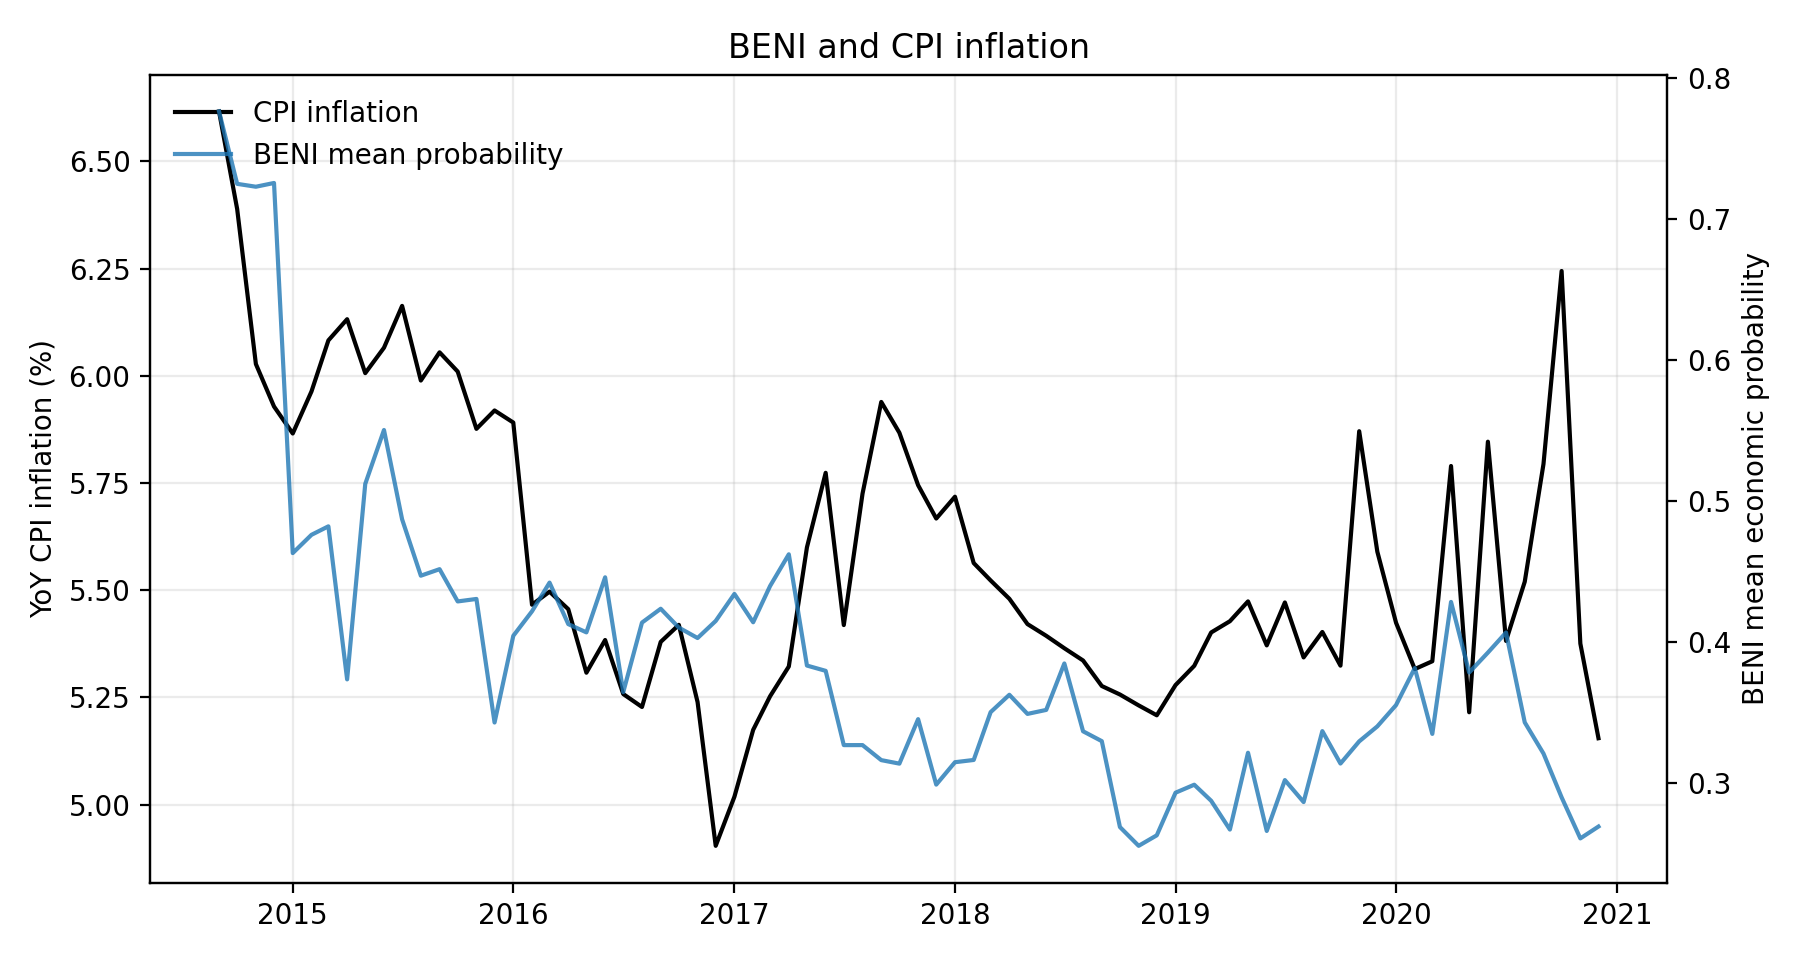
\includegraphics[width=0.9\linewidth]{../results/figures/beni_vs_inflation.png}
\caption{BENI and CPI inflation}
\label{fig:beni_inflation}
\end{figure}

\subsection{Nowcast Fit}

Figure \ref{fig:nowcast} compares actual inflation with AR and AR+BENI same-month forecasts. The BENI-augmented forecast tracks the AR forecast closely, which explains the small difference in RMSE.

\begin{figure}[ht]
\centering
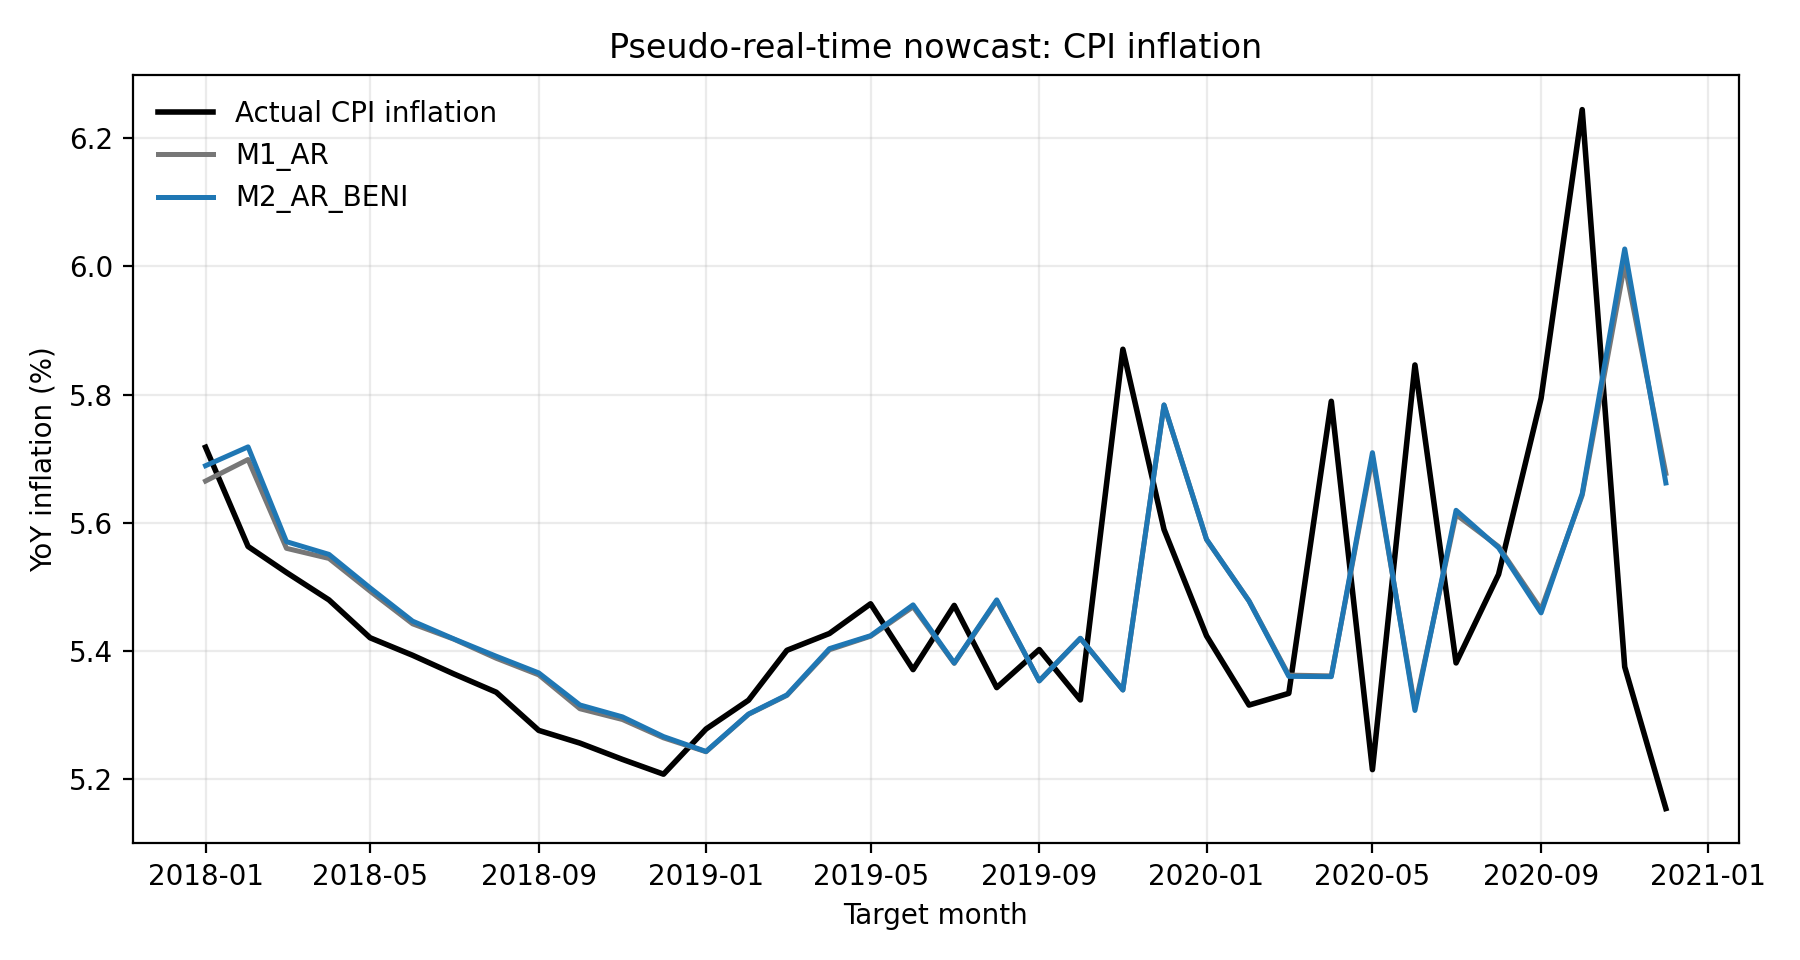
\includegraphics[width=0.9\linewidth]{../results/figures/nowcast_actual_vs_predicted.png}
\caption{Pseudo-real-time nowcasted inflation versus actual inflation}
\label{fig:nowcast}
\end{figure}

\subsection{Asymmetry}

Table \ref{tab:asymmetry} reports forecast errors separately for acceleration, deceleration, and stable-inflation months. The current evidence does not show a clear acceleration advantage for BENI at $h=0$. At $h=3$, AR+BENI modestly improves acceleration and deceleration RMSE relative to AR, but the number of observations is small.

\begin{table}[ht]
\centering
\caption{Forecast performance by inflation regime}
\label{tab:asymmetry}
\begin{tabular}{lrlrrr}
\toprule
model & horizon & regime & n & rmse & mae \\
\midrule
M1\_AR & 0 & acceleration & 17 & 0.251 & 0.178 \\
M2\_AR\_BENI & 0 & acceleration & 17 & 0.253 & 0.178 \\
M3\_AR\_BENI\_FX & 0 & acceleration & 17 & 0.252 & 0.180 \\
M4\_RF\_BENI & 0 & acceleration & 17 & 0.285 & 0.198 \\
M1\_AR & 0 & deceleration & 7 & 0.369 & 0.288 \\
M2\_AR\_BENI & 0 & deceleration & 7 & 0.374 & 0.292 \\
M3\_AR\_BENI\_FX & 0 & deceleration & 7 & 0.385 & 0.300 \\
M4\_RF\_BENI & 0 & deceleration & 7 & 0.375 & 0.289 \\
M1\_AR & 0 & stable & 12 & 0.172 & 0.107 \\
M2\_AR\_BENI & 0 & stable & 12 & 0.174 & 0.110 \\
M3\_AR\_BENI\_FX & 0 & stable & 12 & 0.180 & 0.119 \\
M4\_RF\_BENI & 0 & stable & 12 & 0.172 & 0.128 \\
M1\_AR & 1 & acceleration & 16 & 0.259 & 0.181 \\
M2\_AR\_BENI & 1 & acceleration & 16 & 0.258 & 0.182 \\
M3\_AR\_BENI\_FX & 1 & acceleration & 16 & 0.256 & 0.185 \\
M4\_RF\_BENI & 1 & acceleration & 16 & 0.296 & 0.223 \\
M1\_AR & 1 & deceleration & 7 & 0.330 & 0.244 \\
M2\_AR\_BENI & 1 & deceleration & 7 & 0.348 & 0.255 \\
M3\_AR\_BENI\_FX & 1 & deceleration & 7 & 0.370 & 0.269 \\
M4\_RF\_BENI & 1 & deceleration & 7 & 0.303 & 0.248 \\
M1\_AR & 1 & stable & 12 & 0.182 & 0.142 \\
M2\_AR\_BENI & 1 & stable & 12 & 0.189 & 0.152 \\
M3\_AR\_BENI\_FX & 1 & stable & 12 & 0.222 & 0.184 \\
M4\_RF\_BENI & 1 & stable & 12 & 0.205 & 0.164 \\
M1\_AR & 3 & acceleration & 16 & 0.256 & 0.193 \\
M2\_AR\_BENI & 3 & acceleration & 16 & 0.253 & 0.188 \\
M3\_AR\_BENI\_FX & 3 & acceleration & 16 & 0.248 & 0.195 \\
M4\_RF\_BENI & 3 & acceleration & 16 & 0.291 & 0.221 \\
M1\_AR & 3 & deceleration & 7 & 0.211 & 0.201 \\
M2\_AR\_BENI & 3 & deceleration & 7 & 0.202 & 0.195 \\
M3\_AR\_BENI\_FX & 3 & deceleration & 7 & 0.260 & 0.235 \\
M4\_RF\_BENI & 3 & deceleration & 7 & 0.284 & 0.255 \\
M1\_AR & 3 & stable & 10 & 0.210 & 0.162 \\
M2\_AR\_BENI & 3 & stable & 10 & 0.216 & 0.162 \\
M3\_AR\_BENI\_FX & 3 & stable & 10 & 0.256 & 0.199 \\
M4\_RF\_BENI & 3 & stable & 10 & 0.258 & 0.217 \\
\bottomrule
\end{tabular}

\end{table}

\section{Robustness and Limitations}

The nonlinear random forest model does not improve over the linear AR benchmark in this short sample. Adding exchange-rate change also weakens forecast accuracy in the current setup. These results are consistent with a small-sample warning: the 2018--2020 test window is short, and the TF-IDF BENI prototype may be too coarse to provide clean incremental forecasting information.

The main limitation is that this is not yet the final BENI instrument. Paper 3's human-reviewed labels and BanglaBERT index should replace the TF-IDF index before final submission. English-language benchmark data and food/core CPI should also be added when reliable files are available.

\section{Policy Discussion}

The current results suggest a cautious interpretation. BENI appears useful as a monitoring indicator: it is strongly associated with the inflation environment and can be updated before official CPI is released. However, monitoring value is not the same as nowcasting value. A policy dashboard should therefore present BENI as a narrative pressure indicator alongside, not instead of, official statistical nowcasting models.

\section{Conclusion}

This paper implements the nowcasting evaluation framework for BENI. The preliminary TF-IDF results are mixed: strong level association, weak same-month and one-month forecast gains, and a small three-month improvement. This is a useful benchmark. The final contribution depends on whether the improved Paper 3 BENI index can deliver stronger incremental predictive content under the same pseudo-real-time protocol.

\end{document}
